% short_report.tex — condensed (2-3 page) version of report.tex.
% Numbers pulled from the full report.tex / actual experiment runs against
% this repository's code; see report.tex and scripts/ for full detail.
%
% Compile with: pdflatex short_report.tex (needs pgfplots; run twice for refs).

\documentclass[10pt]{article}
\usepackage[margin=0.85in]{geometry}
\usepackage{booktabs}
\usepackage{hyperref}
\usepackage{amsmath}
\usepackage{pgfplots}
\pgfplotsset{compat=1.17}
\usepackage{xcolor}
\usepackage{enumitem}
\setlist{itemsep=1pt, topsep=2pt, parsep=0pt}
\newcommand{\todo}[1]{\textcolor{red}{\textbf{TODO(you):} #1}}

\title{COL 7364/764 Assignment 1 --- Sparse Retrieval Arena \\ \large Report (Condensed)}
\author{\todo{name and registration number}}
\date{\today}

\begin{document}
\maketitle
\vspace{-1.5em}

\section{Indexing Design}

\textbf{Tokenization/normalization} (\texttt{submission/indexer.py}, \texttt{stemmer.py}):
\begin{itemize}
\item Lowercase alphanumeric regex tokens (\texttt{[a-z0-9]+}) $\to$ stopword removal $\to$ Porter stemming.
\item Porter stemmer implemented \emph{from scratch} (not NLTK): grading runs with \texttt{--network none}, and NLTK's stopword corpus needs a one-time download that would break silently in the container.
\item Verified against classic Porter test vocabulary + textbook over-stemming examples (organization/organ, university/universe).
\item Stopword list: standard 179-word SMART/NLTK English list, embedded directly.
\item Effect (toy set, textbook $k_1,b$): nDCG@10 $0.826\to0.879$, MAP@10 $0.658\to0.825$.
\end{itemize}

\textbf{Persistence \& compression} (\texttt{InvertedIndex.save()/load()}):
\begin{itemize}
\item Stores postings (term$\to$\{doc\_id:tf\}), doc lengths, collection stats. Raw text \emph{not} retained.
\item Doc ids mapped to small integers; postings gap-encoded (delta from previous doc id) and packed with \emph{variable-byte (VByte)} encoding (7-bit groups, high bit = last byte) instead of JSON ASCII digits.
\item Split into 6 single-purpose files; term offsets in \texttt{postings.bin} are never stored --- reconstructed as a running sum of preceding lengths at load time.
\end{itemize}

\begin{table}[h]
\centering\small
\begin{tabular}{lrr}
\toprule
 & JSON (before) & VByte binary (after) \\
\midrule
Index size (171{,}332 docs, trec-covid) & 62.5\,MB & \textbf{29.1\,MB (--53\%)} \\
Build time & 15.2\,s & 16.2\,s \\
Load time & 2.7\,s & 4.4\,s (pure-Python decode loop) \\
\bottomrule
\end{tabular}
\caption{JSON vs.\ VByte persistence. Ranking output bit-identical before/after (round-trip tests in \texttt{tests/test\_index\_persistence.py}). Honest tradeoff: load time up $\sim$60\%, traded for the size win.}
\end{table}

\section{Boolean/VSM vs.\ BM25}

Boolean AND/OR returns an unranked set (not rank-metric-evaluable); used only as a correctness-checked filter. Ranked comparison is TF-IDF cosine VSM vs.\ BM25, same tokenizer/index (\texttt{scripts/compare\_scorers.py}):

\begin{table}[h]
\centering\small
\begin{tabular}{llrrrr}
\toprule
Corpus & Scorer & nDCG@10 & MAP@10 & MRR & P@10 \\
\midrule
toy (20 docs) & BM25 & 0.8826 & 0.8250 & 1.0000 & 0.3167 \\
toy (20 docs) & VSM  & 0.8793 & 0.8250 & 1.0000 & 0.3167 \\
full (171K, trec-covid) & BM25 & \textbf{0.6672} & \textbf{0.0166} & 0.8590 & \textbf{0.7380} \\
full (171K, trec-covid) & VSM  & 0.4425 & 0.0103 & 0.6864 & 0.5060 \\
\bottomrule
\end{tabular}
\caption{Gap negligible on toy set (too small to separate models); large at scale --- BM25's $k_1$/$b$ matter once doc-length/tf distributions actually vary.}
\end{table}

\section{BM25 Parameter Search ($k_1$, $b$)}
\begin{itemize}
\item Swept on \emph{dev} topics/qrels only (never held-out). \texttt{scripts/tune\_bm25.py}: 99 combos, $k_1\in[0.4,3.0]$ (11 vals) $\times$ $b\in[0.0,1.0]$ (9 vals), maximizing nDCG@10.
\item Best: $k_1{=}2.5$, $b{=}0.6$ $\to$ nDCG@10 $=0.6672$, vs.\ $0.6400$ at textbook defaults ($k_1{=}1.2,b{=}0.75$): $+0.027$ absolute.
\item Both curves show an interior peak (not a grid edge) --- some evidence the search range was wide enough.
\item Interpretation: $b{\approx}0.6$ below textbook 0.75 plausibly because trec-covid abstracts are fairly length-uniform vs.\ a mixed newswire corpus, needing less aggressive length normalization. \todo{Confirm with doc-length variance data if time allows.}
\end{itemize}

\begin{figure}[h]
\centering
\begin{minipage}{0.49\textwidth}
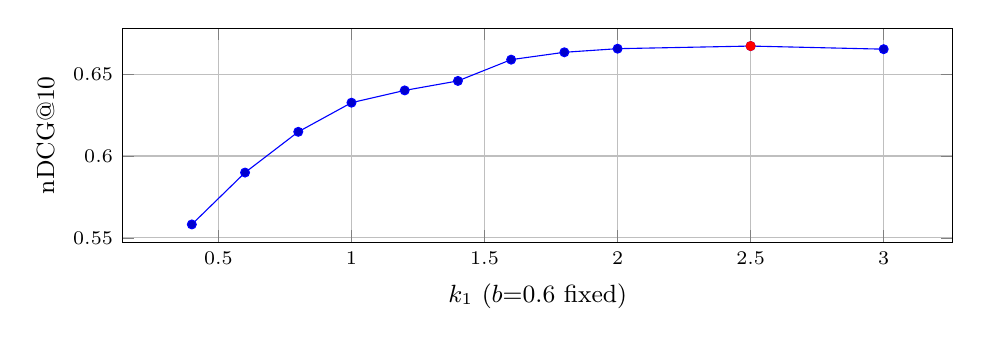
\begin{tikzpicture}
\begin{axis}[width=\textwidth, height=4.3cm, xlabel={$k_1$ ($b{=}0.6$ fixed)}, ylabel={nDCG@10}, grid=major, mark options={scale=0.8}, label style={font=\small}, tick label style={font=\scriptsize}]
\addplot coordinates {(0.4,0.5582)(0.6,0.5899)(0.8,0.6148)(1.0,0.6326)(1.2,0.6401)(1.4,0.6459)(1.6,0.6589)(1.8,0.6634)(2.0,0.6656)(2.5,0.6672)(3.0,0.6653)};
\addplot[only marks, mark=*, red] coordinates {(2.5,0.6672)};
\end{axis}
\end{tikzpicture}
\end{minipage}
\hfill
\begin{minipage}{0.49\textwidth}
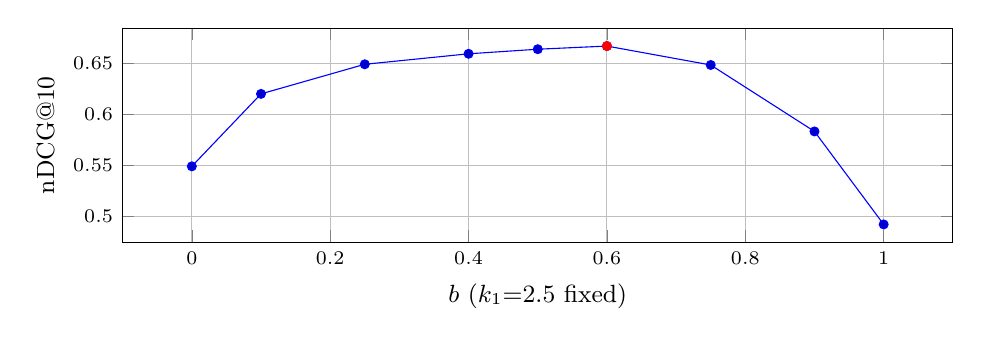
\begin{tikzpicture}
\begin{axis}[width=\textwidth, height=4.3cm, xlabel={$b$ ($k_1{=}2.5$ fixed)}, ylabel={nDCG@10}, grid=major, mark options={scale=0.8}, label style={font=\small}, tick label style={font=\scriptsize}]
\addplot coordinates {(0.0,0.5490)(0.1,0.6202)(0.25,0.6493)(0.4,0.6596)(0.5,0.6641)(0.6,0.6672)(0.75,0.6486)(0.9,0.5833)(1.0,0.4919)};
\addplot[only marks, mark=*, red] coordinates {(0.6,0.6672)};
\end{axis}
\end{tikzpicture}
\end{minipage}
\caption{nDCG@10 vs.\ $k_1$ (left) and $b$ (right), dev set, full trec-covid corpus. Peaks marked.}
\end{figure}

\section{Final Custom Scorer: Static BM25+/VSM Blend}
\texttt{score}$(d) = w\cdot\text{BM25+}_{norm}(d) + (1-w)\cdot\text{VSM}_{norm}(d)$, each min-max normalized to $[0,1]$ per query (BM25 unbounded, VSM already in $[0,1]$). BM25+ (Lv \& Zhai, 2011) adds constant $\delta$ to every matched term's contribution, correcting under-reward of long relevant documents.

\begin{table}[h]
\centering\small
\begin{tabular}{lrr}
\toprule
Configuration & nDCG@10 & MAP@10 \\
\midrule
Plain BM25 ($k_1{=}2.5,b{=}0.6$) & 0.6672 & 0.0166 \\
BM25+VSM blend alone ($w{=}0.75,\delta{=}0$) & 0.6789 & 0.0173 \\
BM25+ alone ($\delta{=}0.1$) & 0.6710 & 0.0170 \\
\textbf{Combined ($\delta{=}0.75,w{=}0.8$)} & \textbf{0.6899} & \textbf{0.0174} \\
\bottomrule
\end{tabular}
\caption{Full \texttt{build\_index/load\_index/retrieve} harness run (\texttt{runs/full\_report.json}). Total gain over plain BM25: $+0.0227$ nDCG@10, on top of $+0.027$ from $k_1$/$b$ tuning.}
\end{table}

\begin{itemize}
\item \textbf{Latency cost}: mean query latency $40.5\to153.8$\,ms initially (redundant sorting in \texttt{custom\_scorer.score()}: two throwaway sorts + one combined sort). Fixed by adding \texttt{raw\_scores()} (unsorted dict) to \texttt{bm25.py}/\texttt{boolean\_vsm.py} and sorting once $\to$ \textbf{105.3\,ms} (--32\%), nDCG@10 unchanged (0.6896).
\item \textbf{Confirmed near-optimal}: joint 4-param grid search ($k_1,b,\delta,w$ together, 81 combos) found the \emph{same} point already reached by staged tuning ($+0.0009$, within noise).
\item \textbf{RRF alternative rejected}: rank-based fusion (Cormack et al., 2009) scored $0.6649$ at best ($k_{rrf}{=}60$) --- worse than the additive blend (0.6892); BM25/VSM raw score magnitudes carry real signal that RRF discards.
\end{itemize}

\section{Explored and Rejected Alternatives}
\begin{table}[h]
\centering\small
\begin{tabular}{p{2.7cm}p{6.4cm}p{4.5cm}}
\toprule
Idea & Result & Decision \\
\midrule
Rocchio PRF (blind query expansion) & Every one of 36 swept configs \emph{worse} than plain BM25; best still $-0.045$ nDCG@10. Topic drift: short medical queries pull in generic co-occurring terms. & Implemented, correct, \textbf{not wired in}. \\
True title/abstract field weighting & Real gain with genuine title metadata ($+0.019$ nDCG@10), but corpus contract guarantees only flat \texttt{text} --- no title. Token-prefix heuristic proxy recovered only 5.5\% of the gain. & \textbf{Not wired in} (no safe fallback). \\
Proper BM25F (single-saturation) & Beats naive two-pass blend by $+0.0077$ with \emph{true} fields (0.6938 vs.\ 0.6861); but \emph{worse} than plain BM25 with the heuristic pseudo-title (0.6576) --- amplifies noisy field data, not just diluting it. Degrades gracefully to title-absent (fiqa, no title attribute): 0.2365 vs.\ plain BM25's 0.2400. & \textbf{Not wired in}; parked pending a real title field. \\
Coordination-level bonus ($\gamma\cdot$ fraction of distinct query terms matched) & Monotonic decline for every $\gamma{>}0$ (0.6897$\to$0.6350 at $\gamma{=}1$). Long natural-language queries penalized for not echoing every word. & Code kept, default $\gamma{=}0$ (exactly reproduces blend). \\
Bigram/phrase proximity bonus & Monotonic decline for every $\mu{>}0$; index size $+227\%$ (30.5MB$\to$99.8MB) for a signal that never helped --- bigram matches too rare/noisy. & \textbf{Fully reverted} (was unconditionally built regardless of $\mu$). \\
\bottomrule
\end{tabular}
\end{table}

\section{Cross-Dataset Generalization Check}
Same unmodified \texttt{retrieve()}, same hardcoded $k_1{=}2.5,b{=}0.6,\delta{=}0.75,w{=}0.8$ (tuned only on trec-covid), run against two unseen BEIR corpora:
\begin{table}[h]
\centering\small
\begin{tabular}{lrrrr}
\toprule
Dataset & Docs & Our nDCG@10 & Local ref.\ nDCG@10 & Margin \\
\midrule
trec-covid (tuning corpus) & 171{,}332 & 0.6892 & 0.4279 & $+61.1\%$ \\
fiqa (financial Q\&A) & 57{,}638 & 0.2467 & 0.1603 & $+53.9\%$ \\
nfcorpus (nutrition) & 3{,}633 & 0.3310 & 0.2682 & $+23.4\%$ \\
\bottomrule
\end{tabular}
\end{table}
\begin{itemize}
\item Largest margin is on the tuning corpus itself (expected); still a solid margin (54\%, 23\%) on two unseen domains/scales --- not overfit to a single corpus.
\item Absolute nDCG@10 lands close to (nfcorpus) or above (fiqa) BEIR-paper BM25 baselines ($\sim$0.32, $\sim$0.236) --- external sanity check.
\end{itemize}

\section{Error Analysis}
\todo{Regenerate against final blended \texttt{retrieve()} --- table below is from plain-BM25 (\S3), before \S5's blend was wired in.}
\begin{table}[h]
\centering\small
\begin{tabular}{p{9cm}rr}
\toprule
Query & nDCG@10 & P@10 \\
\midrule
``what causes death from Covid-19?'' & 0.0948 & 0.10 \\
``best practices in hospitals/home for quarantine?'' & 0.1606 & 0.50 \\
``How does coronavirus differ from seasonal flu?'' & 0.2664 & 0.20 \\
``do recovered individuals show sufficient immune response...'' & 0.2811 & 0.50 \\
``what is the origin of COVID-19'' & 0.3000 & 0.80 \\
\bottomrule
\end{tabular}
\end{table}
\begin{itemize}
\item Since the whole corpus is COVID-related, ``covid''/``coronavirus''/``19'' have near-zero IDF --- ranking driven only by remaining content words.
\item Queries needing a \emph{relationship} between remaining terms (``\emph{causes} death'', not just co-mention) suffer most --- a bag-of-words scorer has no proximity signal. Consistent with why coordination/bigram bonuses were tried (\S6) but both failed empirically.
\item \todo{Manually inspect top-10 doc\_ids vs.\ qrels for 1--2 of these to confirm with a concrete example.}
\end{itemize}

\section{Final Competition Entry}
\todo{Confirm before submission.} \texttt{retrieve()} uses \texttt{submission/custom\_scorer.py}'s static BM25+/VSM blend ($k_1{=}2.5,b{=}0.6,\delta{=}0.75,w{=}0.8$): BM25+ and VSM scores min-max normalized per query and linearly combined. Chosen for a $+0.023$ nDCG@10 gain over plain tuned BM25 at an acceptable latency cost ($\sim$105ms mean). Boolean retrieval is implemented/correct but not on the ranked competition path. Rocchio PRF and true field-weighting were implemented and evaluated but not shipped --- PRF underperformed on every config; field weighting needs a title field the corpus contract doesn't guarantee.

\section{AI-Use Disclosure Statement}
\todo{Confirm/complete --- must be accurate for every session, not just this one.} Claude Code (Anthropic) was used as a development assistant across multiple sessions. In the report-drafting session: the Porter stemmer/stopword list, the BM25 parameter sweep and $k_1$/$b$ choice, the Rocchio PRF implementation and its rejection, VByte index compression, accompanying unit tests, and this report were written with Claude Code's assistance under the student's direction and review. \todo{An earlier session (git commit \texttt{40108e5}) produced the initial \texttt{bm25.py}/\texttt{boolean\_vsm.py} --- describe that session's AI use from memory.}

\section{Code Provenance Statement}
\todo{Confirm/complete.} Porter stemming follows Porter (1980), \emph{Program} 14(3) --- from-scratch implementation, not copied, verified against canonical test vocabulary. Stopword list: standard 179-word SMART/NLTK list. VByte encoding follows Manning/Raghavan/Sch\"utze \S5.3.2 (standard technique, not copied). BM25, TF-IDF/cosine VSM, Boolean AND/OR, the inverted index, and Rocchio PRF are original implementations of published formulas (Robertson \& Walker 1992; Robertson \& Zaragoza 2009; Rocchio 1971), with no external search/indexing library used.

\end{document}
